\chapter{Theory}

The following chapter shortly introduces the theoretical background of the experimental methods used in this work, namely \ac{XPS} and \ac{NIXSW}. For more detailed information, please refer to the cited literature.


\section{X-ray photoelectron spectroscopy (XPS)}

\Acf{XPS} is based on the photoelectric effect, which is the ejection of electrons from bound states to the continuum by photon excitation.\autocite{Hertz1887, Einstein1905} The photon energies of X-rays ($E_\mathrm{\gamma}=h\nu$) are similar to the \acf{BE} $E_\mathrm{B}$ of core electrons in atoms. Often, soft X-rays with energies between \SI{100}{\eV} and \SI{2100}{\eV} are used to excite core electrons into the vacuum level. More precisely, $E_\mathrm{\gamma}$ for each core level is chosen to be higher than the respective \ac{BE} in order to create photoelectrons with a kinetic energy $E_\mathrm{kin}$ of approximately \SI{100}{\eV}. The specific choice of $E_\mathrm{\gamma}$ leads to a high surface sensitivity of the technique, as the mean free path of the emitted photoelectrons is only a few nanometers.\autocite{Fairley2021}

The photoemission process is schematically illustrated in \autoref{fig:XPS-schematic}. Incident X-ray photons are absorbed by a core level electron (here: 1s electron), which leads to the ejection of a photoelectron. The kinetic energy of the emitted photoelectron $E_\mathrm{kin}$ is the difference between the tunable photon energy of the X-rays $E_\mathrm{\gamma}$ and the \ac{BE} $E_\mathrm{B}$ of the core level electron in its initial state. This kinetic energy of the emitted photoelectron is measured by an analyzer and provides information about the chemical environment and the oxidation state of the atom. This phenomenon is referred to as chemical shift.\autocite{Kolasinski2012}

\begin{figure}[htb]
	\centering
	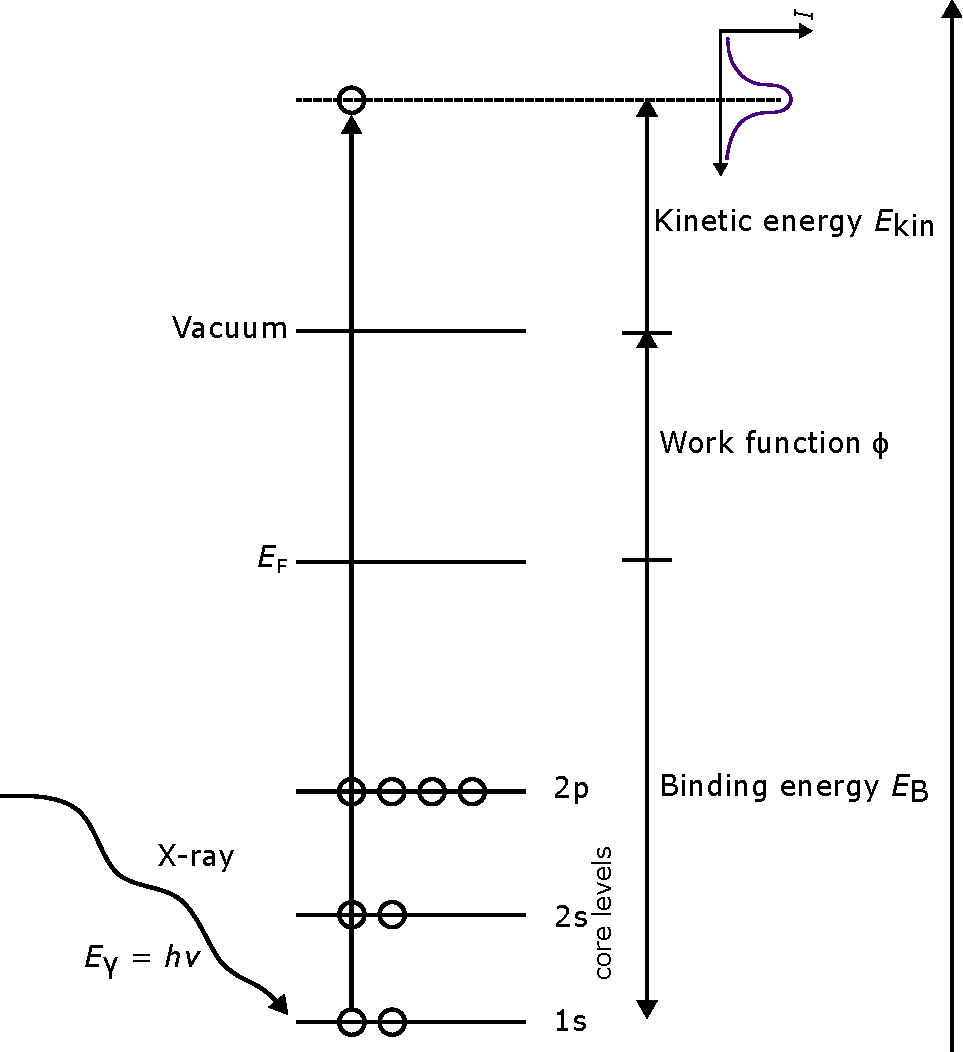
\includegraphics[width=0.7\textwidth]{images/vertiefer/XPS_schematic.pdf}
	\caption{Schematic drawing of the photoemission process of an electron in the 1s orbital upon X-ray excitation. The image was adapted using reference \cite{Attard1998}.}
	\label{fig:XPS-schematic}
\end{figure}

The kinetic energy of the emitted photoelectron that is measured by the analyzer $E'_\mathrm{kin}$ is relative to the Fermi level and given by:

\begin{equation}
	\label{eq:KineticEnergy2}
	E'_\mathrm{kin} = E_\mathrm{kin} + \phi_\mathrm{sample},
\end{equation}

where $E_\mathrm{kin}$ is the kinetic energy of the photoelectron and $\phi_\mathrm{sample}$ is the work function of the sample. As seen in \autoref{fig:XPS-schematic}, the kinetic energy of the emitted photoelectron can be expressed as:

\begin{equation}
	\label{eq:KineticEnergy}
	E_\mathrm{kin} = E_\mathrm{\gamma} - E_\mathrm{B} - \phi_\mathrm{sample},
\end{equation}

where $E_\mathrm{\gamma}=h\nu$ is the photon energy of the incident X-rays and $E_\mathrm{B}$ is the \ac{BE} of the core level electron in its initial state.

$E_\mathrm{B}$ of an electron is defined as the energy difference between the final state of the system $E_\mathrm{f}(n-1)$ and the initial state of the system $E_\mathrm{i}(n)$ with $n$ electrons:

\begin{equation}
    \label{eq:BindingEnergy}
    E_\mathrm{B}=E_\mathrm{f}(n-1)-E_\mathrm{i}(n).
\end{equation}

As seen in \autoref{eq:BindingEnergy}, \ac{BE} depends on initial state and final state effects.

The initial state effects occur for the neutral unexcited atome and are determined by the chemical environment of the atom. Final state effects result from the ionized final state due to the photoemission process. Furthermore, as the photoemission process is fast, the system may not be in an adabatic equilibrium.\autocite{Woodruff2016}

In addition, asymmetric line shapes of the photoemission spectra result from coupling of the emitted photoelectron to the conduction electrons.\autocite{Moulder1993} Moreover, various other effects have a large effect on the line shapes and \ac{FWHM} of the photoemission spectra, such as phonon broadening, the lifetime of the photohole, the spectral resolution of the exciting X-ray beam and the energy resolution of the analyzer.\autocite{Fairley2021,Moulder1993}

\newpage
\section{Normal Incidence X-ray Standing Wave (NIXSW)}

\Acf{NIXSW} is a technique that is based on \ac{XPS} and allows to determine the positions of atoms relative to the Bragg planes of a substrate lattice with chemical sensitivity.\autocite{Zegenhagen1993,Woodruff1998,Woodruff2016,Jones2002}

In contrast to other \ac{XSW} techniques, \ac{NIXSW} is measured with an angle of the incoming X-rays that is close to $\theta_\mathrm{B}=90°$ with respect to the Bragg plane. This is necessary for the investigation of molecules on metal substrates. The reason behind this is that the Bragg condition $2 d_\mathrm{hkl} \sin(\theta_\mathrm{B})=n\lambda$ is essentially unaffected by small angular deviations for $\theta_\mathrm{B}\approx 90°$, because the gradient with respect to $\theta_\mathrm{B}$ is very small. This unsensitivity to angular deviations is needed because metal substrates have a lower degree of perfection compared to semiconductor substrates, which is caused by the higher mosaicity of the metal substrate.\autocite{Zegenhagen1993,Woodruff1998,Woodruff2016}

\begin{figure}[htbp]
	\centering
	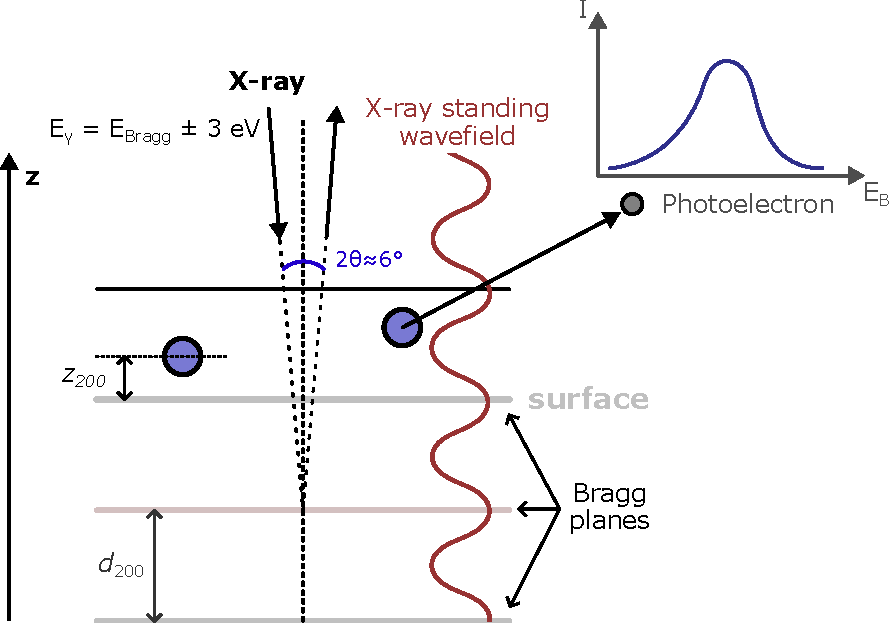
\includegraphics[width=0.85\textwidth]{images/NIXSW-theo.pdf}
	\caption{Schematic drawing of the principle of \ac{NIXSW}. The image was adapted using reference \cite{Woodruff1998}.}
	\label{fig:NIXSW-schematic}
\end{figure}

The principle of \ac{NIXSW} is schematically illustrated in \autoref{fig:NIXSW-schematic}. An incoming X-ray beam is reflected at the surface of a single crystal substrate and interferes with the incoming beam, which leads to an standing wavefield. The standing wavefield extends into the bulk material and also into the vacuum above the surface.\autocite{Woodruff1998} The periodicity of the standing wavefield is given by the spacing $d_\mathrm{hkl}$ of the Bragg planes of the substrate lattice. As there is a small difference between the incoming and the reflected X-ray beam, the intensity of the reflected beam as a function of the wavelength $\lambda$ (or respective beam energy $E_\mathrm{\gamma}=h\frac{c}{\lambda}$) can be measured, which is referred to as reflectivity curve. 

The intensity of the reflected X-ray beam depends on the photon energy $E_\mathrm{\gamma}$. This is illustrated in \autoref{fig:reflectivity}. As the photon energy $E_\mathrm{\gamma}$ is tuned through the Bragg energy $E_\mathrm{B}$, the anti-nodes of the standing wavefield shift with a phase $\nu(E_\mathrm{\gamma})$ from $\pi$ to 0 with higher photon energies. For low photon energies $E_\mathrm{\gamma}$, the anti-nodes of the standing wavefield are located between the Bragg planes. As the photon energy $E_\mathrm{\gamma}$ is increased, the anti-nodes of the standing wavefield shift by $d_\mathrm{hkl}/2$ and are directly located at theBragg planes. Accordingly, the absorption of the X-rays by the atoms of the substrate increases with a higher overlap of the anti-nodes of the standing wavefield with the Bragg planes, which leads to a decrease in the intensity of the reflected X-ray beam. This results in the characteristic asymmetric line shape of the reflectivity curve, which is known as the Darwin-Prins curve.\autocite{Prins1930,Darwin1914}

\begin{figure}[htbp]
	\centering
	\begin{subfigure}[b]{0.48\textwidth}
		\centering
		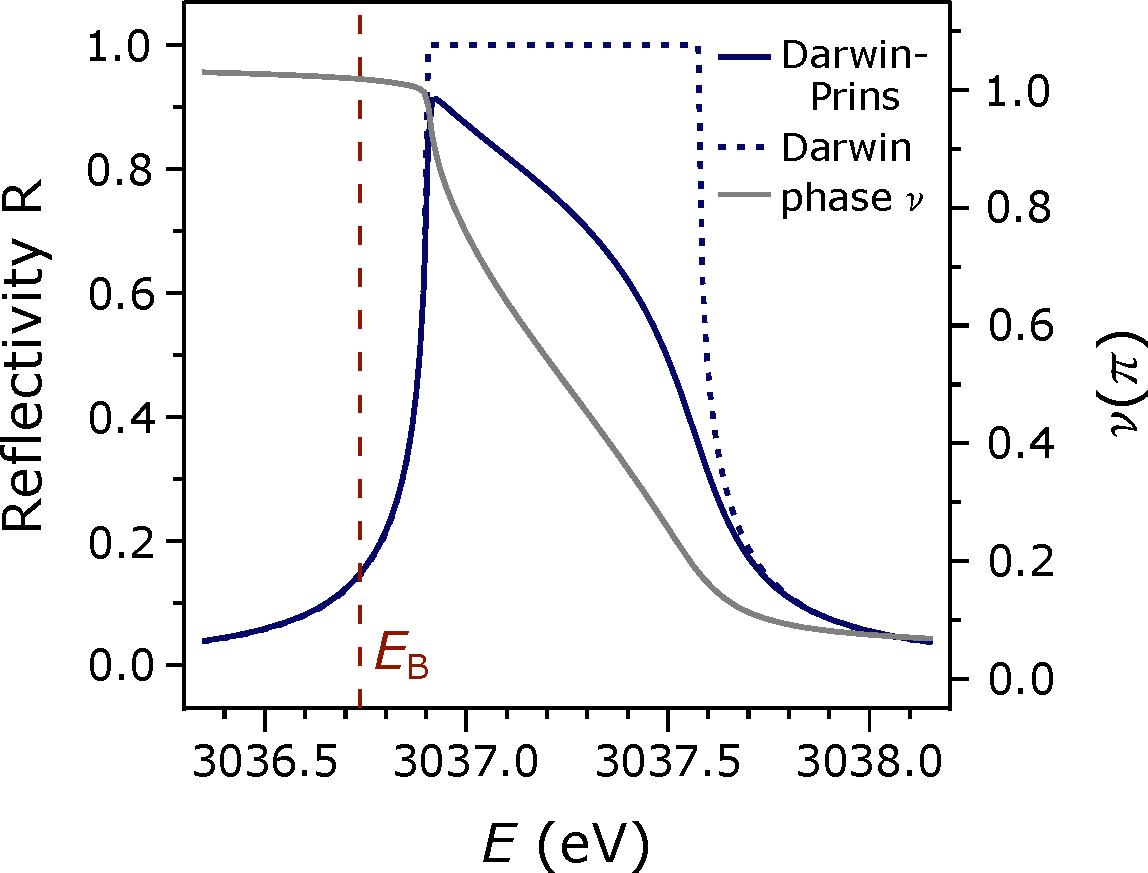
\includegraphics[width=\textwidth]{images/Reflectivity.pdf}
		\caption{Reflectivity curve showing the intensity of the reflected X-ray beam as a function of photon energy.}
		\label{fig:reflectivity}
	\end{subfigure}
	\hfill
	\begin{subfigure}[b]{0.48\textwidth}
		\centering
		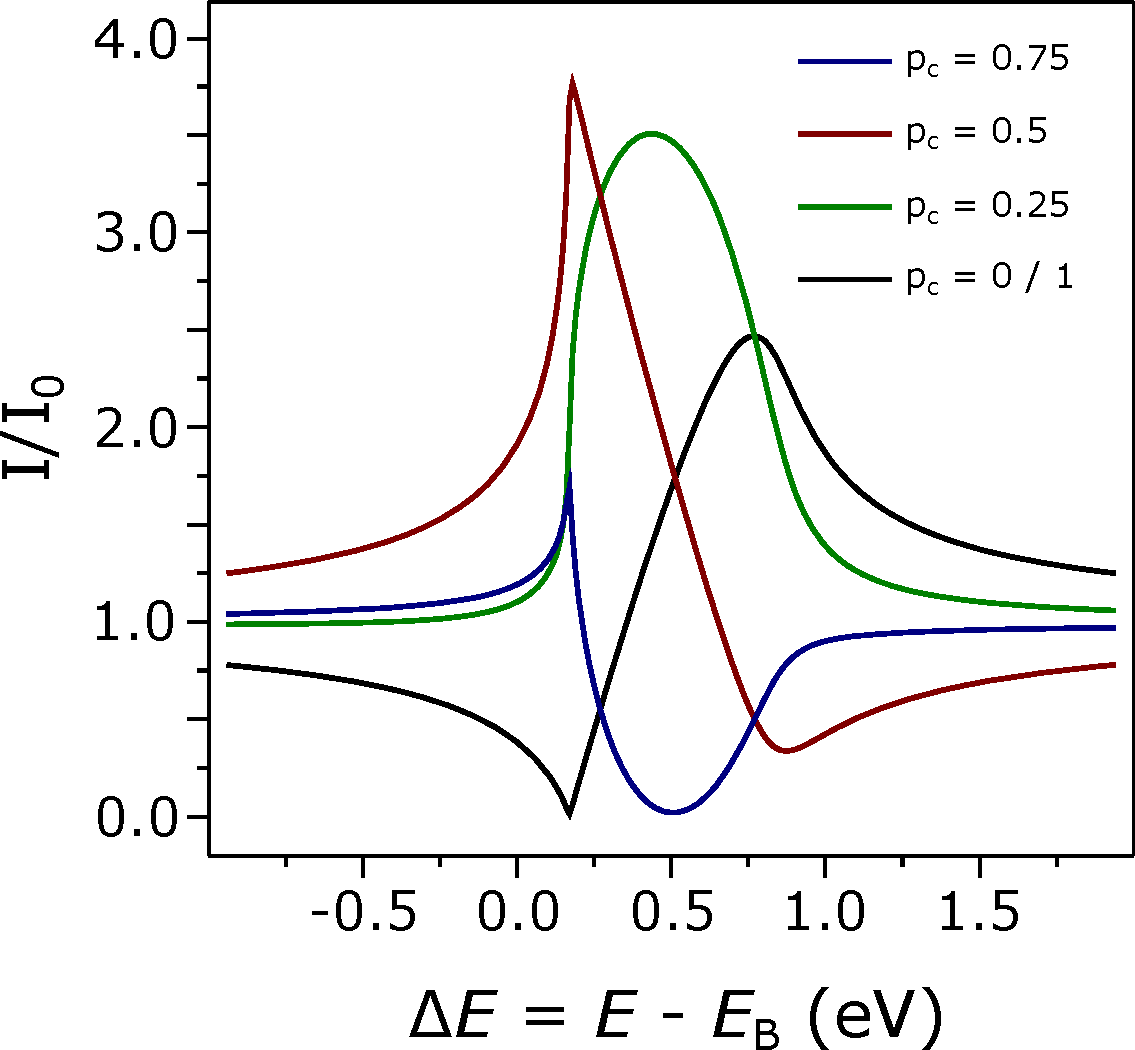
\includegraphics[width=\textwidth]{images/Yield.pdf}
		\caption{Photoelectron yield showing the modulation of photoemission intensity due to the standing wave field.}
		\label{fig:yield}
	\end{subfigure}
	\caption{Illustrated as in reference \cite{Bauer2014}.}
	\label{fig:refl-yield}
\end{figure}

Depending on the position of the absorbed atoms relative to the Bragg plane, the atoms experience different intensities of the standing wavefield, which can be measured by e.g. \ac{XPS}. The change of the photoemission intensity due to the standing wavefield is referred to as photoelectron yield and is schematically illustrated in \autoref{fig:yield}. The normalized photoemission yield $\frac{I}{I_0}$ can be expressed as:

\begin{equation}
	\label{eq:Yield}
	\frac{I}{I_0} = 1 + R(E_\mathrm{\gamma}) + 2\sqrt{R(E_\mathrm{\gamma})} f_\mathrm{c} \cos(\nu(E_\mathrm{\gamma}) - 2\pi p_\mathrm{c}),
\end{equation}

where $R(E_\mathrm{\gamma})$ is the reflectivity, $\nu(E_\mathrm{\gamma})$ is the phase of the standing wavefield, $f_\mathrm{c}$ is the coherent fraction and $p_\mathrm{c}$ is the coherent position.

The coherent fraction $f_\mathrm{c}$ is a measure of the degree of order of the adsorbed atoms and can take values between 0 and 1. A value of $f_\mathrm{c}=1$ indicates that all atoms are located at the same vertical distance relative to the Bragg plane, while a value of $f_\mathrm{c}=0$ indicates that the atoms are randomly distributed.

In addition, the coherent position $p_\mathrm{c}$ is a measure of the average vertical distance of the adsorbed atoms relative to the Bragg plane and can take values between 0 and 1. A value of $p_\mathrm{c}=0$ indicates that the atoms are located at the Bragg plane, while a value of $p_\mathrm{c}=0.5$ indicates that the atoms are located halfway between two Bragg planes. The coherent position $p_\mathrm{c}$ can be converted into the adsorption height $z$ of the adsorbed atoms relative to the substrate surface by the following equation:

\begin{equation}
	\label{eq:NIXSW-height}
	z = (n + p_\mathrm{c}) d_\mathrm{hkl},
\end{equation}

where $n$ is an integer and equals 1 for the (200) Bragg reflection of the Ag(100) substrate used in this work.

However, \autoref{eq:Yield} does not take into account non-dipolar effects, which can lead to a deviation of the measured photoelectron yield. These non-dipolar effects can be accounted for by the following equation:

\begin{equation}
	\label{eq:YieldNonDipolar}
	\frac{I}{I_0} = 1 + S_\mathrm{R} R(E_\mathrm{\gamma}) + 2 |S_\mathrm{I}| \sqrt{R(E_\mathrm{\gamma})} f_\mathrm{c} \cos(\nu(E_\mathrm{\gamma}) - 2\pi p_\mathrm{c} + \psi),
\end{equation}

where $S_\mathrm{R}$, $|S_\mathrm{I}|$ and $\psi$ iare non-dipolar correction parameters, which can be calculated from the scattering phase shifts $\delta p$ and $\delta d$.\autocite{Bocquet2019,Jablonski2010}


\cleardoublepage